\documentclass{article}
\usepackage{amsmath}
\usepackage[english]{babel}
\usepackage[utf8]{inputenc}
\usepackage[a4paper, margin=2.5cm]{geometry} 
\usepackage{geometry}
\usepackage{titlesec}
\usepackage{enumitem} 
\usepackage{xcolor}
\usepackage{hyperref}
%\usepackage{pdfpages}
\usepackage{graphicx}


\title{Workshop 1}
\author{Henry Ricaurte Mora 20221020084}
\date{}

\begin{document}

\maketitle

\section{Introducción}
Este es un documento de prueba para verificar la correcta compilación de LaTeX.


\section*{Components: }

\begin{itemize}[leftmargin=*]
    \item \textbf{\textbf{Mouse}}: It is the first input. It is necessary for the functioning of the analyzed system.
    \item \textbf{\textbf{Hover}}, \textbf{\textbf{Click}}: Functions that are part of the first input.
    \item \textbf{\textbf{X}}, \textbf{\textbf{Y}}: Cartesian location of each of the inputs within the system.
    \item \textbf{\textbf{Event\_handler}}: Group responsible for handling each of the individual events of the system.
    \item \textbf{\textbf{Name}}: Name of each event in the system.
    \item \textbf{\textbf{Text}}: Text associated with each event in the system.
    \item \textbf{\textbf{Session\_id}}: Unique identifier of the session.
    \item \textbf{\textbf{User\_id}}: Unique identifier of the user within the system.
    \item \textbf{\textbf{Level}}: User parameter that characterizes their skill level and/or progress.
    \item \textbf{\textbf{Login\_interface}}: Interface that functions as an input to access the system.
    \item \textbf{\textbf{Auth\_system}}: Authentication system to determine whether access is granted or denied.
    \item \textbf{\textbf{Configuration}}: Component responsible for managing the game's configurations.
    \item \textbf{\textbf{Hq}}: Identifier related to the visual configuration of the system.
    \item \textbf{\textbf{Full\_screen}}: Identifier related to the visual configuration of the system.
    \item \textbf{\textbf{Option\_music}}: Component that balances the game’s music.
    \item \textbf{\textbf{Screen}}: Specifies characteristics related to the program’s magnitude.
    \item \textbf{\textbf{Audio\_system}}: External system component that provides the user with specific game audio.
    \item \textbf{\textbf{Music\_room}}: Component responsible for the music in the room.
    \item \textbf{\textbf{Music\_game}}: Component responsible for the game’s music.
    \item \textbf{\textbf{Id\_notebook}}: Unique identifier of the notebook.
    \item \textbf{\textbf{Pages}}: Space for making notes, paraphrasing ideas, or building a solution.
    \item \textbf{\textbf{Event\_registry}}: Registry of all events in the system.
    \item \textbf{\textbf{Data\_analystic}}: Component responsible for generating and managing the system’s solution to reach the objective.
    \item \textbf{\textbf{Performance}}: Main output of the system (not feedback-based).
\end{itemize}

\section*{Relationships}

Our first relationship is the one related to the \textbf{\textbf{login\_interface}}, 
which leads us to an \textbf{\textbf{auth\_system}} that is responsible for either returning a 
credential error or performing a login and modeling the system based on a \textbf{\textbf{user\_id}}.
\\
\\
As a primary relationship, we have the one that generates the input: the \textbf{\textbf{mouse}}, 
which contains two main events: \textbf{\textbf{hover}} and \textbf{\textbf{click}}, where each 
of these is mapped using a Cartesian coordinate (\textbf{\textbf{x}}, \textbf{\textbf{y}}). This 
first "major" system constantly communicates by sending all information 
to the \textbf{\textbf{event\_handler}}, which contains a \textbf{\textbf{name}} and 
a \textbf{\textbf{text}} for each of these events.
\\
\\
Continuing with the design of the user interface system, after entering the
 \textbf{\textbf{user\_id}}, it obtains a \textbf{\textbf{level}}, which is responsible for 
 setting in relation to the \textbf{\textbf{user\_id}}. This same \textbf{\textbf{user\_id}} 
 component implements a \textbf{\textbf{configuration}} and creates a \textbf{\textbf{session\_id}},
  which is then responsible for sharing that information with the \textbf{\textbf{event\_handler}}.
  \\
  \\
Approaching the \textbf{\textbf{configuration}} section, we have 3 relationships that obtain state
 information and share it with the corresponding components: \textbf{\textbf{hq}},
  \textbf{\textbf{full\_screen}}, and \textbf{\textbf{option\_music}}. Both \textbf{\textbf{hq}} 
  and \textbf{\textbf{full\_screen}} send information to the \textbf{\textbf{screen}} as output.
  \\
  \\
\textbf{\textbf{Option\_music}} also generates an output to the \textbf{\textbf{audio\_system}},
 and in addition, is able to receive what other components such as \textbf{\textbf{music\_room}}
 and \textbf{\textbf{music\_game}} transmit, and make changes by generating a turn 
 \textbf{\textbf{off}} or \textbf{\textbf{on}}.
 \\
 \\
In \textbf{\textbf{user\_id}} we also handle another relationship: this one gets to 
\textbf{\textbf{id\_notebook}}’s component, which contains \textbf{\textbf{pages}} 
that are connected with an event we will manage as \textbf{\textbf{event\_handler}}.
\\
\\
\textbf{\textbf{Event\_handler}} is an important component since it adds everything it receives 
to another component called \textbf{\textbf{event\_registry}}, which is in charge of handling all 
event records. These are then \textbf{\textbf{sent\_to}} the \textbf{\textbf{data\_analystic}}’s 
component, which generates a \textbf{\textbf{performance}} of the analyzed system.

\section*{Model}
\begin{center}
    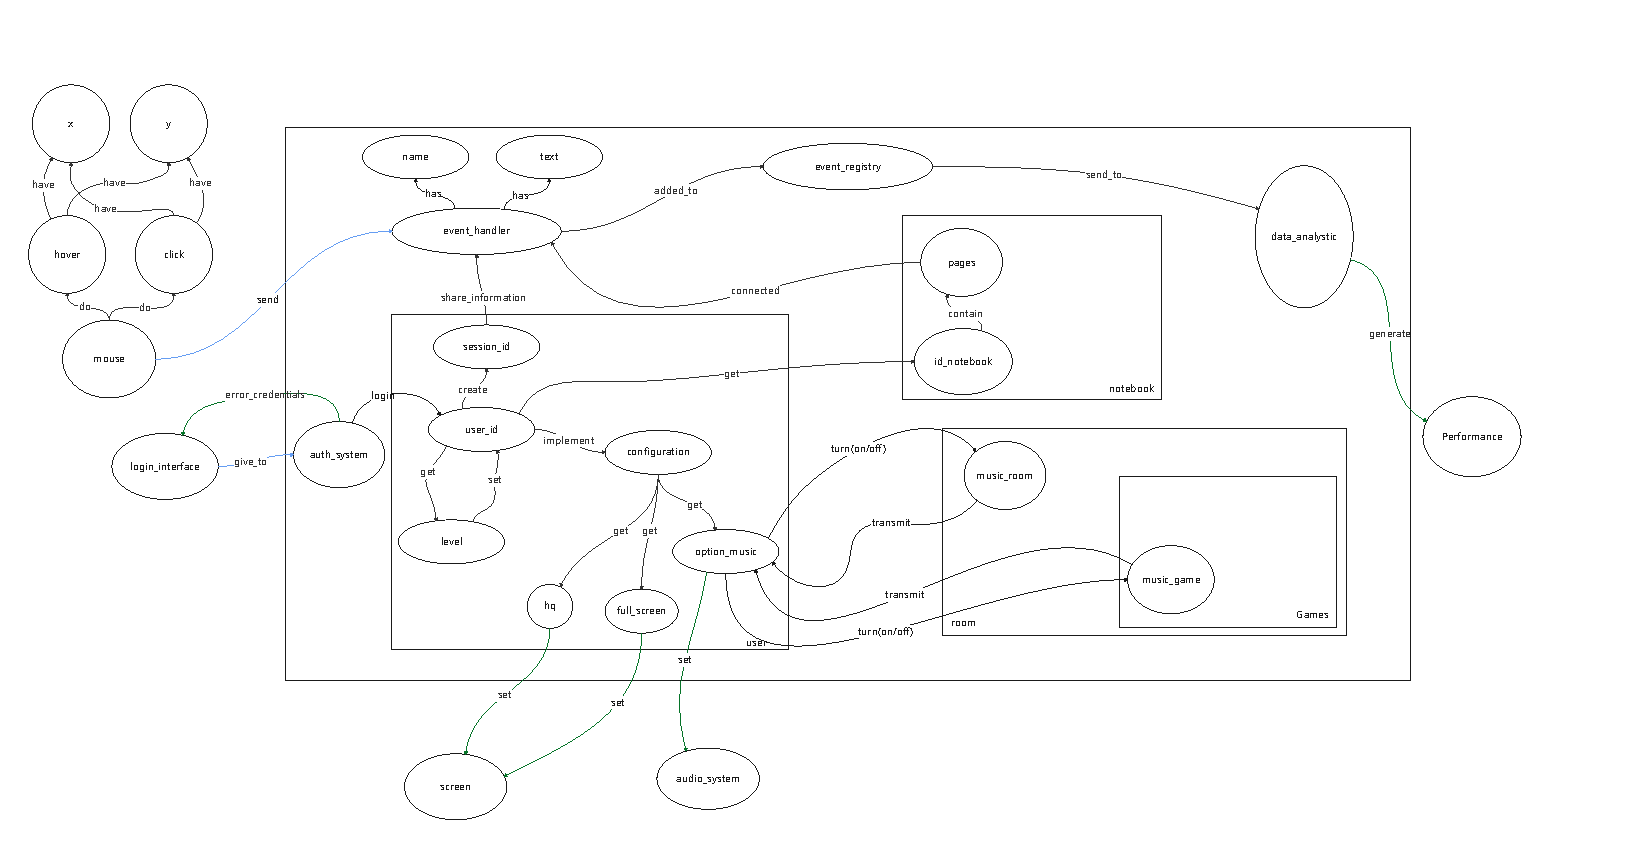
\includegraphics[width=0.75\textwidth]{src/IO.pdf}
  \end{center}
\end{document}
